\documentclass[crop,tikz]{standalone}

\usepackage{pgfplots}
\pgfplotsset{compat=1.18}

\begin{document}
  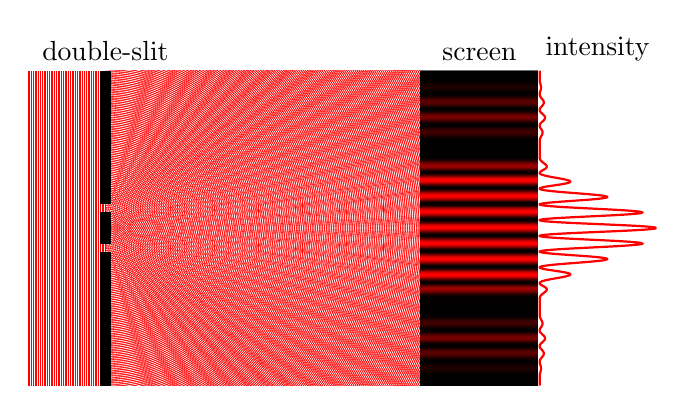
\begin{tikzpicture}
    \pgfmathsetmacro{\xmax}{2*pi}; % max. x value in plot (indirectly determines the wavelength)
    \pgfmathsetmacro{\maxz}{0.1}; % max. z value in 2-dim intensity plot
    \pgfmathsetmacro{\maxheight}{4}; % max. plot height H
    \pgfmathsetmacro{\screendistance}{4}; % screen distance L
    \pgfmathsetmacro{\plotwidth}{3}; % width of plot
    \pgfmathsetmacro{\slitwidth}{0.1}; % width b of slits
    \pgfmathsetmacro{\doverb}{5}; % ratio of slit distance d / slit width b = d/b
    \pgfmathsetmacro{\slitdistance}{\doverb*\slitwidth}; % slit distance d
    % xmax/Pi Sqrt[1 + (2L/H)^2]
    \pgfmathsetmacro{\boverlambda}{\xmax/pi*sqrt(1 + (2*\screendistance/\maxheight)^2)}; % ratio slit width b / wavelength lambda = b/lambda
    \pgfmathsetmacro{\wavelength}{\slitwidth/\boverlambda}; % wavelength
    % plane wave
    \foreach[parse=true] \ncircle in {0,1,...,{1/\wavelength}} {
      \draw[red,very thin] ({-\ncircle*\wavelength},{-\maxheight/2}) -- ++ (0,{\maxheight});
    }
    % circular waves
    \begin{scope}
      \clip (0,{-\maxheight/2}) rectangle ({\screendistance},{\maxheight/2});
      \foreach[parse=true] \ncircle in {1,2,...,{0+sqrt(\screendistance^2 + \maxheight^2)/\wavelength}} {
        \draw[red,very thin] (0,{-\slitdistance/2 - \ncircle*\wavelength}) arc (-90:90:{\ncircle*\wavelength});
        \draw[red,very thin] (0,{+\slitdistance/2 - \ncircle*\wavelength}) arc (-90:90:{\ncircle*\wavelength});
      }
    \end{scope}
    % double-slit
    \draw[line width=4pt]
      (0,{-\maxheight/2}) -- (0,{-\slitdistance/2 - \slitwidth/2})
      (0,{-\slitdistance/2 + \slitwidth/2}) -- (0,{\slitdistance/2 - \slitwidth/2})
      (0,{\slitdistance/2 + \slitwidth/2}) -- (0,{\maxheight/2});
    % screen
    \begin{axis}[
      width={\maxheight*1cm},
      height={\plotwidth*1cm},
      scale only axis,
      anchor=origin,
      rotate around={-90:(current axis.origin)},
      yshift=4cm,
      axis lines=none,
      view = {0}{90},
      xmin={-\xmax}, xmax={\xmax},
      ymin=0, ymax=2.02,
      zmin=0, zmax={\maxz},
      domain={-\xmax}:{\xmax},
      samples=1000,
      colormap={blackred}{rgb=(0,0,0) rgb=(1,0,0)},
      ]
      % 1-dim intensity
      \addplot[red,thick,smooth] (x,{1.02 + 0.25*(sin(deg(x))/x)^2 * (sin(deg(2*\doverb*x))/sin(deg(\doverb*x)))^2});
      % 2-dim intensity
      \addplot3[surf,domain y=0:1,samples y=2,shader=flat,colormap name=blackred] {min(\maxz,(sin(deg(x))/x)^2) * (sin(deg(2*\doverb*x))/sin(deg(\doverb*x)))^2};
    \end{axis}
    % labels
    \node[above] at (0,{\maxheight/2}) {double-slit};
    \node[above] at ({\screendistance + \plotwidth/4},{\maxheight/2}) {screen};
    \node[above] at ({\screendistance + 3*\plotwidth/4},{\maxheight/2}) {intensity};
  \end{tikzpicture}
\end{document}
